\section{Mechanism-1 Complete Reference}

\subsection{Source Objects}
Mechanism-1 contains exactly six original source objects and 48 tasks.
The objects are not imported OMR models and are not random spatial
crops. They were authored as coherent systems with recognizable
functional modules.

\begin{figure*}[t]
\centering
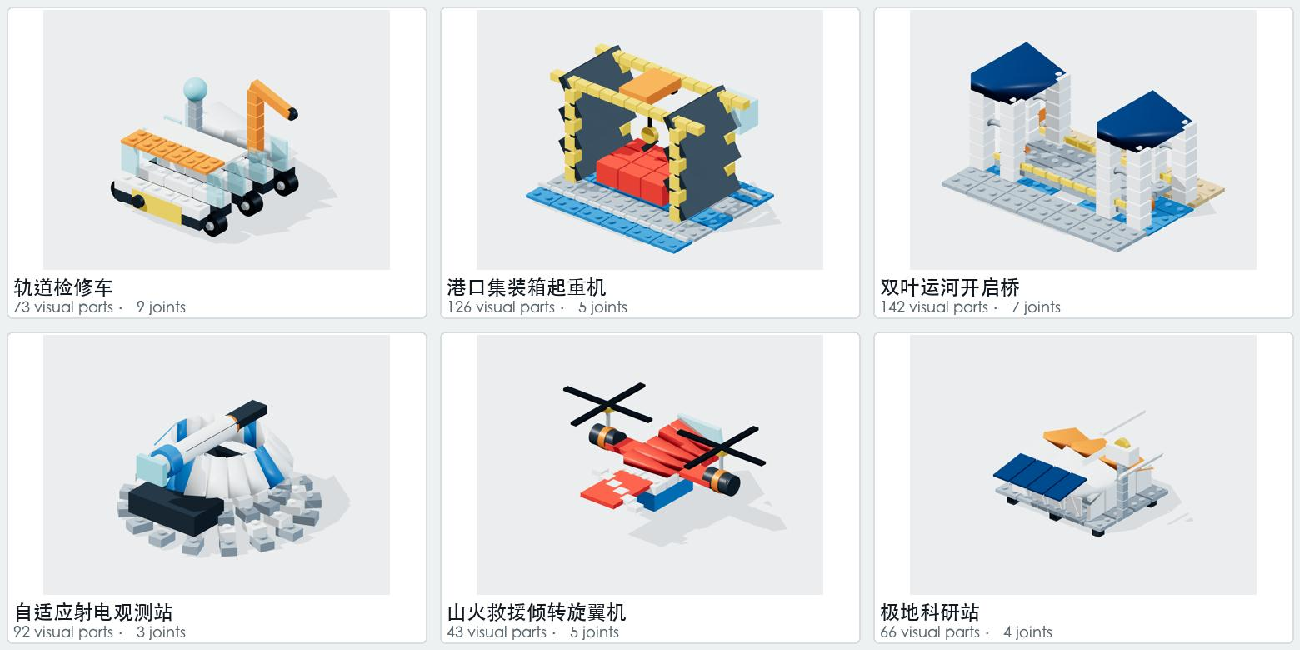
\includegraphics[width=\textwidth]{figures/mechanism-models.pdf}
\caption{The complete Mechanism-1 source set. Each object contributes
all eight task families, so task count never increases the number of
independent source objects.}
\label{fig:supp-mechanism-models}
\end{figure*}

\begin{table}[H]
\centering\small
\begin{tabular}{lrrr}
\toprule Object & Parts & Modules & Joints\\
\midrule
\tableinput{tables/mechanism-models.tex}
\bottomrule
\end{tabular}
\caption{Source-object composition. Visible parts are grouped into
compound rigid modules for physics.}
\end{table}

\paragraph{Orbital Service Rover.}
Six wheels, a pressure cabin, battery cartridge, panoramic mast and
articulated sampling arm support wheel/axle, service-access and arm-joint
reasoning.
\paragraph{Harbor Container Crane.}
A rail foundation, braced twin tower, prismatic trolley, vertical hoist,
hook latch and container create coupled access, payload and recovery tasks.
\paragraph{Bascule Canal Gate.}
Two bridge towers, hinged leaves, counterweight gears and a drive
cartridge separate final geometry from movable-deck function.
\paragraph{Adaptive Radio Observatory.}
A terraced base, rotating segmented dome, elevation telescope and
cryogenic camera create two-axis kinematic and service problems.
\paragraph{Wildfire Tiltrotor.}
Twin tilting nacelles, independent rotors, wing, fuselage and removable
water tank create functional and dynamic failure modes.
\paragraph{Polar Research Station.}
An elevated insulated building, airlock, sliding solar carriage and
wind rotor create access, weather-load and maintenance tasks.

\subsection{Task Contracts}
\begin{figure*}[t]
\centering
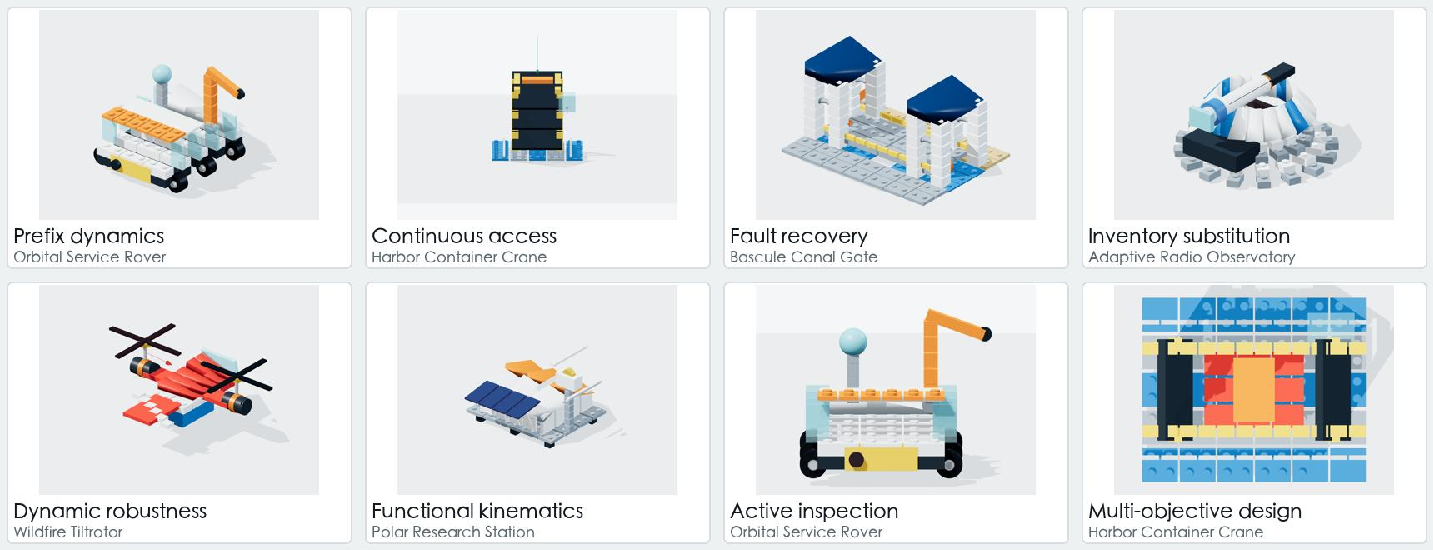
\includegraphics[width=\textwidth]{figures/mechanism-tasks.pdf}
\caption{One rendered example from every Mechanism-1 family.
The release browser contains all 48 task renders, public inputs,
oracles, and model answers.}
\label{fig:supp-mechanism-tasks}
\end{figure*}

\paragraph{Prefix dynamics.}
Two module sequences are submitted without evaluator reordering.
For every prefix, the simulator instantiates available modules and
joints, advances one second under gravity, and records displacement.
The output identifies the fully valid plan and the first failing
zero-based prefix of the other.

\paragraph{Insertion access.}
A service tool is represented by a cuboid envelope. Rapier casts that
shape continuously along each candidate path while the serviced module
is removed. The exact set of collision-free path IDs is required.
This differs from endpoint collision or 2D occlusion.

\paragraph{Fault recovery.}
A declared joint is removed, the simulation returns child displacement
and tilt, and the model selects the causal joint plus an ordered minimum
repair sequence. A correct joint with incomplete or reordered actions
does not pass.

\paragraph{Inventory substitution.}
Four replacement strategies expose piece count, cost, mass, stiffness
and connection mode. The selected alternative must satisfy all hard
limits; visual similarity is irrelevant.

\paragraph{Dynamic robustness.}
After settling, an off-center impulse is applied to a named module.
Equivalent motion is the maximum of translation and radius-scaled
rotation. The answer is the largest tested impulse meeting both transient
and residual limits.

\paragraph{Functional kinematics.}
The simulator actuates a named revolute or prismatic joint toward a
target. Some visually valid systems fail because of load, limits or
interference. The model predicts the measured pass/fail result rather
than merely naming the joint.

\paragraph{Active inspection.}
Four hidden worlds encode nominal, reversed, missing-brace and jammed
states. Candidate observations and costs are explicit. The output is
the query maximizing expected information gain per unit cost.

\paragraph{Multi-objective design.}
Candidates trade cost, mass and stiffness. The answer must contain the
complete non-dominated set; selecting one preferred design is not enough.

\subsection{Physics Reproduction}
The release uses \texttt{@dimforge/rapier3d-compat} 0.20.0
(Apache-2.0), a 120\,Hz fixed step, 12 solver iterations and two
internal PGS iterations. Model and task generation is deterministic.
The visual vocabulary includes bricks, plates, beams, panels, slopes,
arches, windows, wheels, axles, gears, cylinders and spheres.

The simulator creates compound colliders for each rigid module.
Fixed, revolute and prismatic joints use public anchors, axes and limits.
Motor targets, impulses and shape casts are stored in public inputs.
Slope and arch colliders are conservative cuboid envelopes and therefore
may reject a path that a higher-fidelity mesh would accept; this is
recorded as a limitation.

\subsection{Measured Model Results}
\begin{table*}[t]
\centering\small
\begin{tabular*}{\textwidth}{@{}l@{\extracolsep{\fill}}rrrrrrrr@{}}
\toprule
Model & Prefix & Access & Repair & Stock & Dynamics & Function & Inspect & Pareto\\
\midrule
\tableinput{tables/mechanism-results.tex}
\bottomrule
\end{tabular*}
\caption{Exact successes out of six source objects per family.
The local Qwen baseline is text-only; GPT and Gemini receive one task
render. All responses have valid JSON format.}
\end{table*}

GPT-4.1 mini obtains 28/48, Gemini 2.5 Flash 31/48, and local
Qwen3-0.6B 3/48. The cloud models solve 5/6 and 6/6 prefix cases,
and both solve all stock questions. GPT/Gemini obtain 3/6 and 3/6 on access, 0/6 and 3/6 on
exact repair, 5/6 and 2/6 on dynamics, 3/6 and 3/6 on function,
4/6 and 4/6 on inspection, and 2/6 and 4/6 on complete Pareto sets.

The paid run contains 96 calls and costs \$0.069427. Temperature is
zero, automatic retries and provider fallback are disabled, and the
same image/structured evidence is used for both cloud models. These
are descriptive development results over six public source clusters.

\subsection{Artifacts and Boundaries}
The static browser \texttt{mechanism-v1/index.html} exposes every model,
question, capability label, public input, oracle and model response.
\texttt{CASEBOOK.zh-CN.md} provides the same information in Chinese.
The release also includes raw API outputs, local-model outputs,
per-task scores, 72 rendered frames and hash manifests.

Rapier evidence does not calibrate commercial-brick clutch, ABS
deformation, manufacturing tolerance, wear, robot grasping or human
ergonomics. OMR/LDraw models remain under
\texttt{references/omr-design-reference} as design references only;
they never enter Mechanism-1 tasks, splits, model prompts or scores.
